<<<<<<< HEAD
%Preamble
\documentclass[11pt,oneside,letterpaper]{article}

=======
\documentclass[11pt,oneside,letterpaper]{article}

% graphicx package, useful for including eps and pdf graphics
\usepackage{graphicx}
\DeclareGraphicsExtensions{.pdf,.png,.jpg}

% basic packages
\usepackage{color}
\usepackage{parskip}
\usepackage{float}

>>>>>>> 9e83a793b72db391a6823d211e00a08aed8f21c8
% text layout
\usepackage{geometry}
\geometry{textwidth=15cm} % 15.25cm for single-space, 16.25cm for double-space
\geometry{textheight=22cm} % 22cm for single-space, 22.5cm for double-space

<<<<<<< HEAD
% make links a more pleasing color and don't box them
\usepackage{color}
\definecolor{green}{rgb}{0.20,0.50,0.48}
\usepackage[hidelinks]{hyperref}
\hypersetup{colorlinks=true,linkcolor=black,citecolor=black,urlcolor=green}

\usepackage{parskip}

\usepackage{authblk}
\usepackage[utf8]{inputenc}
\usepackage[T1]{fontenc}
\usepackage{amsmath}
\usepackage{amssymb}
\usepackage{amsthm}
\usepackage{amsfonts}
\usepackage{mathrsfs}
\usepackage{mathtools}
\usepackage{enumerate}
\usepackage[shortlabels]{enumitem}
\usepackage{verbatim} %% includes comment environment
\usepackage[capitalize]{cleveref}
\crefformat{equation}{~(#2#1#3)}
\usepackage{graphicx}
\usepackage{mathrsfs}

% cite package, to clean up citations in the main text
\usepackage{cite}
=======
% helps to keep figures from being orphaned on a page by themselves
\renewcommand{\topfraction}{0.85}
\renewcommand{\textfraction}{0.1}
>>>>>>> 9e83a793b72db391a6823d211e00a08aed8f21c8

% bold the 'Figure #' in the caption and separate it with a period
% Captions will be left justified
\usepackage[labelfont=bf,labelsep=period,font=small]{caption}

<<<<<<< HEAD
% can include this for journal submission to help with reviewer feedback, but don't include for preprint
% \usepackage{lineno}
% \linenumbers
% \linespread{1.5} % Increase Line spread

\renewcommand{\vec}[1]{\boldsymbol{#1}}

\title{Placeholder}

\author[1,2,*]{Eslam Abousamra}
\author[1,3,*]{Marlin Figgins}
\author[1,4]{Trevor Bedford}
\affil[1]{Vaccine and Infectious Disease Division, Fred Hutchinson Cancer Research Center, Seattle, WA, USA}
\affil[2]{Department of Epidemiology, University of Washington, Seattle, WA, USA}
\affil[3]{Department of Applied Mathematics, University of Washington, Seattle, WA, USA}
\affil[2]{Howard Hughes Medical Institute, Seattle, WA, USA}

\affil[*]{Co-first authors}
\date{\today}
%Figure out author affilations...
% https://maehler.se/blog/2013/11/01/authors-and-affiliations-in-latex
=======
% review layout with double-spacing
%\usepackage{setspace}
%\doublespacing
%\captionsetup{labelfont=bf,labelsep=period,font=doublespacing}

% cite package, to clean up citations in the main text. Do not remove.
\usepackage{cite}
%\renewcommand\citeleft{(}
%\renewcommand\citeright{)}
%\renewcommand\citeform[1]{\textsl{#1}}

% Remove brackets from numbering in list of References
\renewcommand\refname{\large References}
\makeatletter
\renewcommand{\@biblabel}[1]{\quad#1.}
\makeatother

\usepackage{authblk}
\renewcommand\Authands{ \& }
\renewcommand\Authfont{\normalsize \bf}
\renewcommand\Affilfont{\small \normalfont}
\makeatletter
\renewcommand\AB@affilsepx{, \protect\Affilfont}
\makeatother

% notation
\usepackage{amsmath}
\usepackage{amssymb}

%%% TITLE %%%
\title{\vspace{1.0cm} \Large \bf
ncov-forecasting-fit (title TBD)
}

\author[1,2]{Eslam Abousamra}
\author[1,3]{Marlin Figgins}
\author[1,2,4]{Trevor Bedford}

\affil[1]{Vaccine and Infectious Disease Division, Fred Hutchinson Cancer Center, Seattle, WA, USA}
\affil[2]{Department of Epidemiology, University of Washington, Seattle, WA, USA}
\affil[3]{Department of Applied Mathematics, University of Washington, Seattle, WA, USA}
\affil[4]{Howard Hughes Medical Institute, Seattle, WA, USA}

\date{}
>>>>>>> 9e83a793b72db391a6823d211e00a08aed8f21c8

\begin{document}

\maketitle

<<<<<<< HEAD
\begin{abstract}
    The ncov-forecasting-fit repository hosts a data curation and a live-forecasting framework to process pathogen variant data at time-stamped intervals. 
    The framework is built to standardize and estimate accurate real-time nowcast and forecast targets and to facilitate comparisons of forecasting and nowcasting accuracy between different statistical models.
    Using the framework, the purpose of the study is to work with live surveillance data to investigate the empirical side of evolutionary forecasting including growth advantages, frequencies estimates, and cases and to provide a scoring framework of different modelling approaches.
\end{abstract}


\section*{Introduction}

\section*{Results}

\section*{Methods}

\section*{Discussion}

\section*{Conclusion}

\cite{Champredon2018}

=======
%%% ABSTRACT %%%
\begin{abstract}

Todo

\end{abstract}

%%% INTRODUCTION %%%
\section*{Introduction}

I use Google Scholar format for citation style with first author, year and first word of title, ala \cite{hadfield2018nextstrain}.

%%% METHODS %%%
\section*{Methods}

Todo

%%% RESULTS %%%
\section*{Results}

I put figures into a `/figures' directory and use semantic labeling ala (Figure~\ref{example_predictions}).

%%% map %%%
\begin{figure}[h]
	\centering
	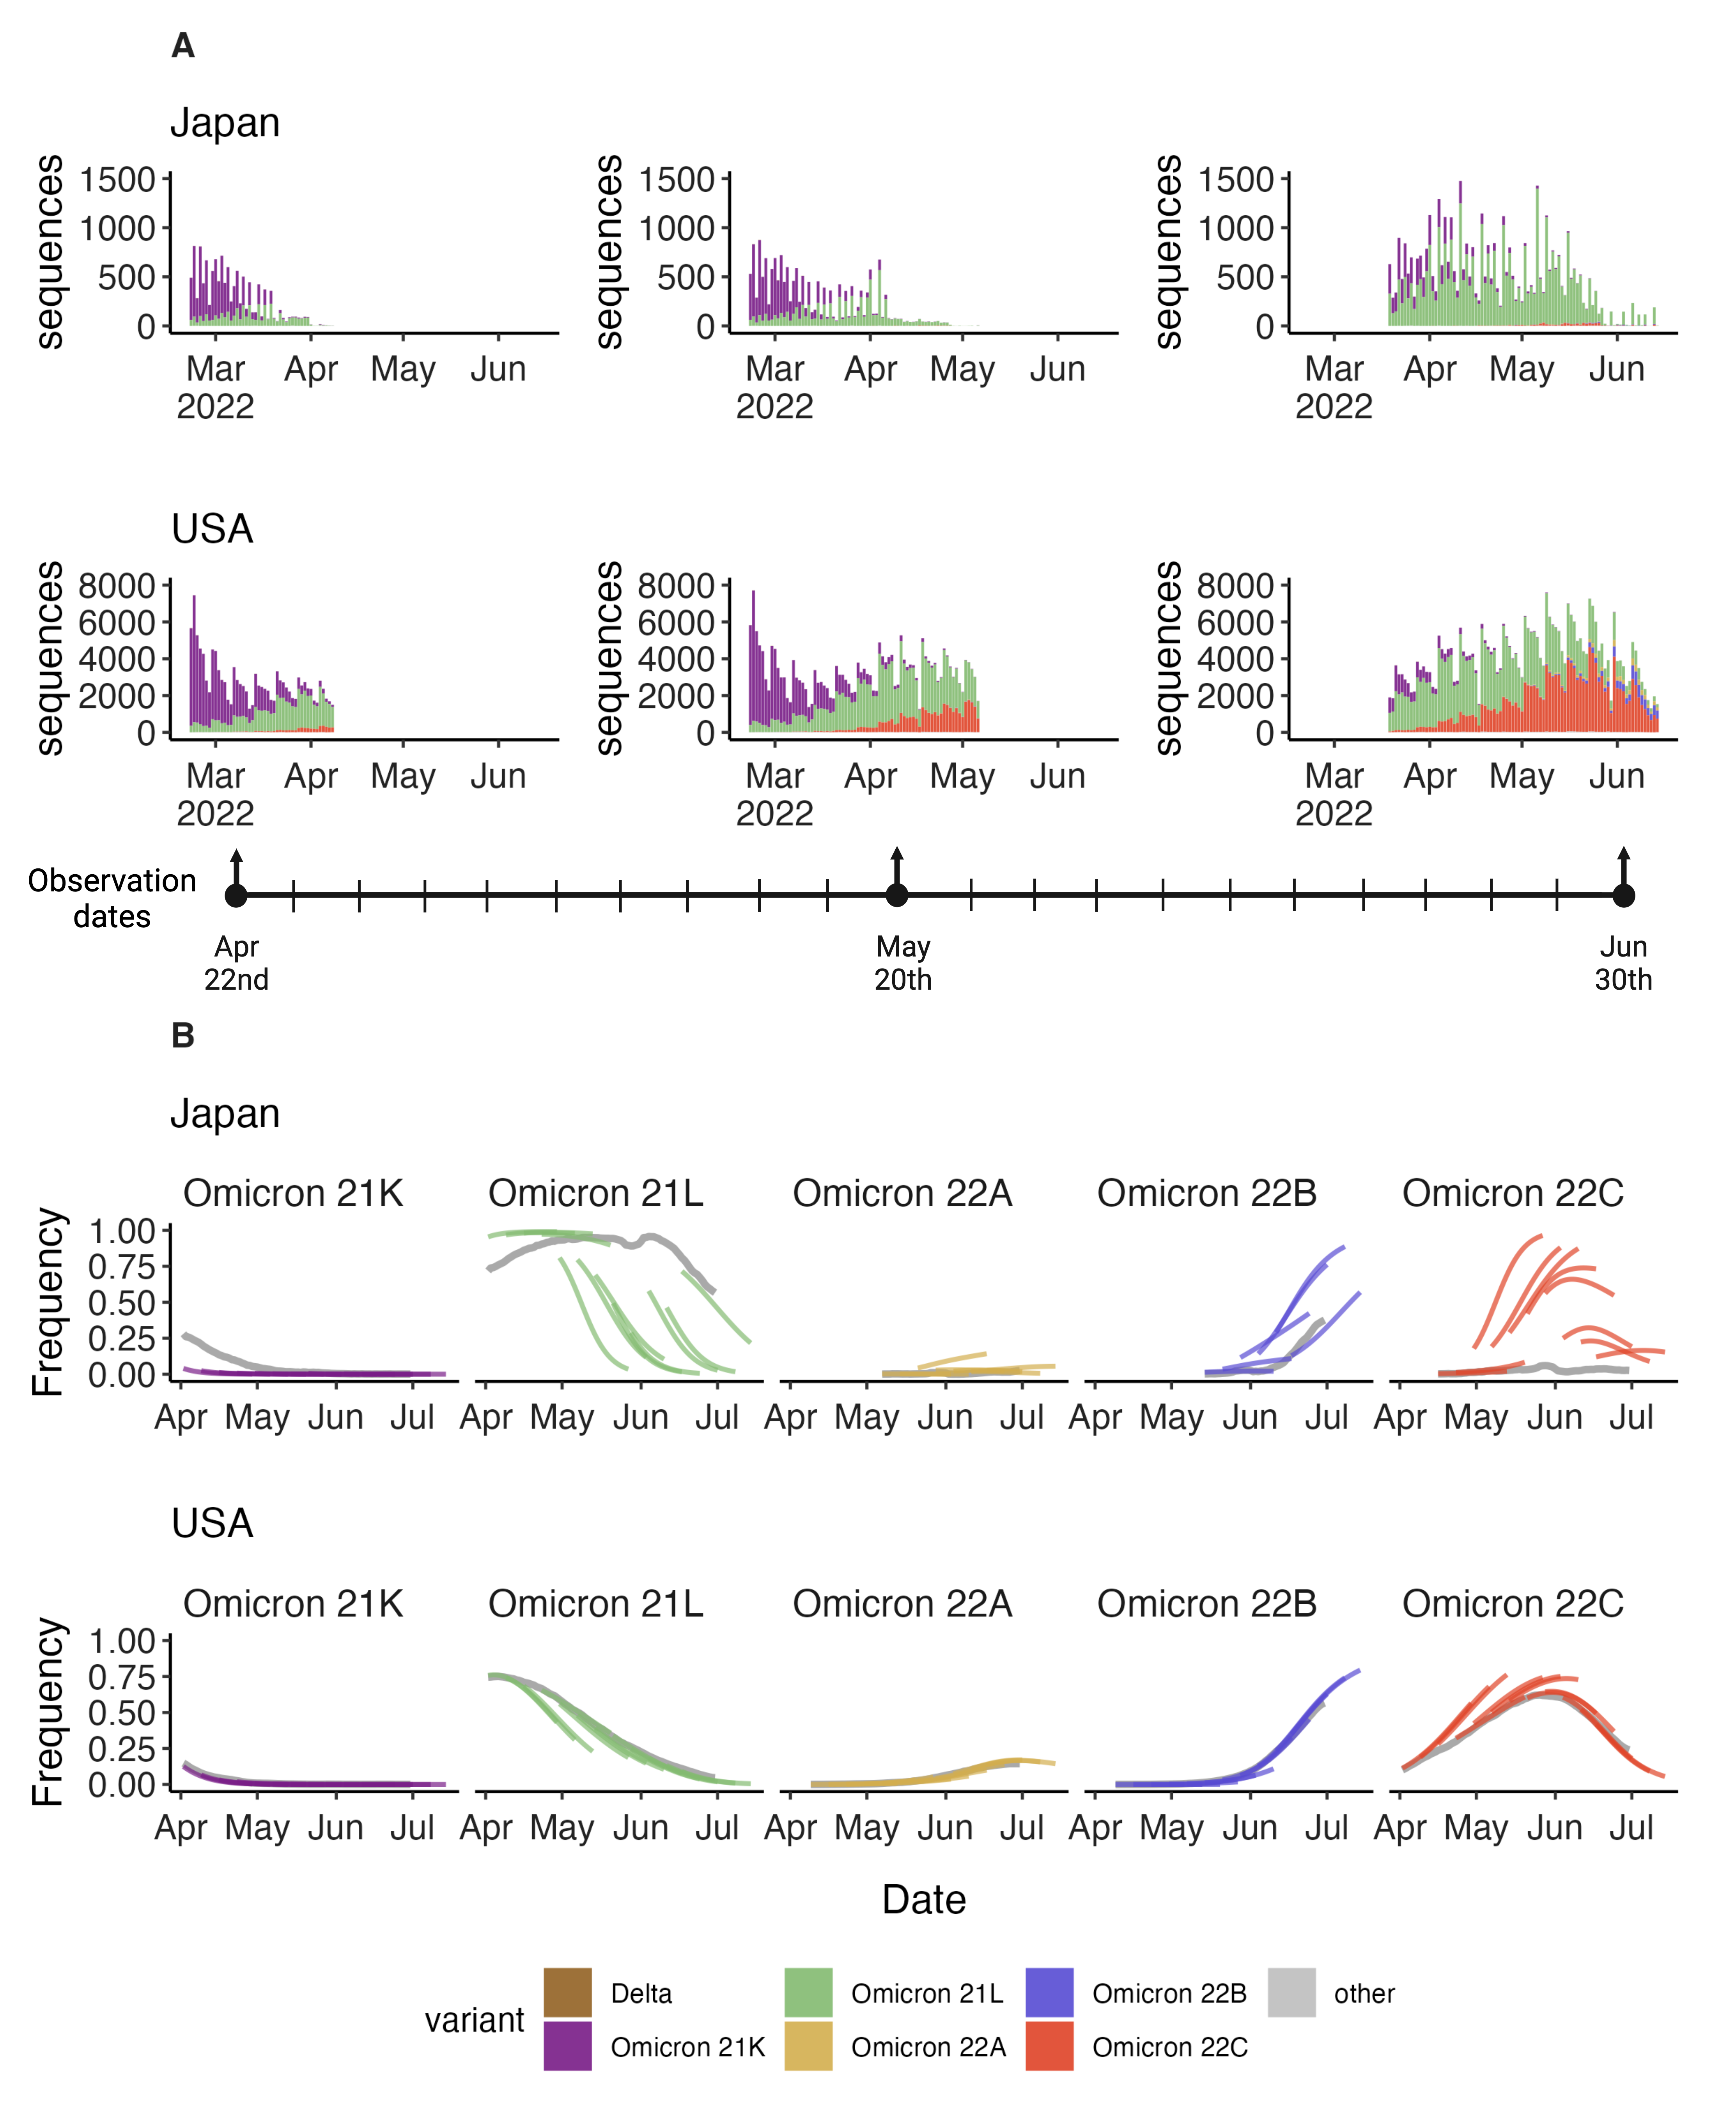
\includegraphics[width=1.0\textwidth]{figures/example_predictions}
	\caption{\textbf{Example data and predictions for Japan and the USA.}
	Further legend here.
	}
	\label{example_predictions}
\end{figure}

%%% DISCUSSION %%%
\section*{Discussion}

Todo

%%% REFERENCES %%%
>>>>>>> 9e83a793b72db391a6823d211e00a08aed8f21c8
\bibliographystyle{plos}
\bibliography{ncov-forecasting-fit}

\end{document}
